\pdfminorversion=4
\documentclass[aspectratio=169]{beamer}

\mode<presentation>
{
  \usetheme{default}
  \usecolortheme{default}
  \usefonttheme{default}
  \setbeamertemplate{navigation symbols}{}
  \setbeamertemplate{caption}[numbered]
  \setbeamertemplate{footline}[frame number]  % or "page number"
  \setbeamercolor{frametitle}{fg=white}
  \setbeamercolor{footline}{fg=black}
} 

\usepackage[english]{babel}
\usepackage[utf8x]{inputenc}
\usepackage{tikz}
\usepackage{courier}
\usepackage{array}
\usepackage{bold-extra}
\usepackage{minted}
\usepackage[thicklines]{cancel}
\usepackage{fancyvrb}

\xdefinecolor{dianablue}{rgb}{0.18,0.24,0.31}
\xdefinecolor{darkblue}{rgb}{0.1,0.1,0.7}
\xdefinecolor{darkgreen}{rgb}{0,0.5,0}
\xdefinecolor{darkgrey}{rgb}{0.35,0.35,0.35}
\xdefinecolor{darkorange}{rgb}{0.8,0.5,0}
\xdefinecolor{darkred}{rgb}{0.7,0,0}
\definecolor{darkgreen}{rgb}{0,0.6,0}
\definecolor{mauve}{rgb}{0.58,0,0.82}
\definecolor{titlecolor}{rgb}{0.25,0.34,0.74}

\title[2020-07-06-scipy2020]{\textcolor{titlecolor}{Manipulating JSON-like Data with NumPy-like Idioms}}
\author{\underline{Jim Pivarski}, Ianna Osborne, Peter Elmer}
\institute{Princeton University -- IRIS-HEP}
\date{July 7, 2020}

\usetikzlibrary{shapes.callouts}

\begin{document}

\logo{\pgfputat{\pgfxy(0.11, 7.4)}{\pgfbox[right,base]{\tikz{\filldraw[fill=dianablue, draw=none] (0 cm, 0 cm) rectangle (50 cm, 1 cm);}\mbox{\hspace{-8 cm}
\includegraphics[height=1 cm]{princeton-logo-long.png}\hspace{0.1 cm}\raisebox{0.1 cm}{
\includegraphics[height=0.8 cm]{iris-hep-logo-long.png}}\hspace{0.1 cm}}}}}

\begin{frame}
  \vspace{1.75 cm}
  \mbox{ } \hfill 
\includegraphics[width=0.4\linewidth]{logo-600px.png} \hfill \mbox{ }
  
  \vspace{-1 cm}
  \titlepage
\end{frame}

\logo{\pgfputat{\pgfxy(0.11, 7.4)}{\pgfbox[right,base]{\tikz{\filldraw[fill=dianablue, draw=none] (0 cm, 0 cm) rectangle (50 cm, 1 cm);}\mbox{\hspace{-8 cm}
\includegraphics[height=1 cm]{princeton-logo.png}\hspace{0.1 cm}\raisebox{0.1 cm}{
\includegraphics[height=0.8 cm]{iris-hep-logo.png}}\hspace{0.1 cm}}}}}

% Uncomment these lines for an automatically generated outline.
%\begin{frame}{Outline}
%  \tableofcontents
%\end{frame}

% START START START START START START START START START START START START START

%% Window capture
%% Crop top: 10
%% Crop left: 15
%% Crop right: 25
%% Crop bottom: 50

%% Audio capture
%% -10.1 dB

%% JupyterLab zoom: 200%

\begin{frame}[fragile]{What do I mean by {\it that}?}
\vspace{0.3 cm}

\small
\begin{minted}{python}
>>> import awkward1 as ak
>>> import numpy as np
\end{minted}

\begin{minted}{python}
>>> dataset = [
...     [{"x": 1,  "y": [101]},
...      {"x": 4,  "y": [102, 202]},
...      {"x": 9,  "y": [103, 203, 303]}],
...     [],
...     [{"x": 16, "y": [104, 204, 304, 404]},
...      {"x": 25, "y": [105, 205, 305, 405, 505]}]
... ]
>>> array = ak.Array(dataset)
\end{minted}

\begin{uncoverenv}<2->
\begin{minted}{python}
>>> array[2, :, "y", -1]
<Array [404, 505] type='2 * int64'>
\end{minted}
\end{uncoverenv}

\begin{uncoverenv}<3->
\begin{minted}{python}
>>> array[:, :, "y", 0] - np.sqrt(array[:, :, "x"])
<Array [[100, 100, 100], [], [100, 100]] type='3 * var * float64'>
\end{minted}
\end{uncoverenv}
\end{frame}

\begin{frame}{Table of contents}
\vspace{0.4 cm}

\large
\begin{description}\setlength{\itemsep}{0.15 cm}
\item[1:00\hspace{0.5 cm}] \textcolor{gray}{(This table of contents)}
\item[2:00\hspace{0.5 cm}] Why does this library exist? Motivation from particle physics
\item[5:00\hspace{0.5 cm}] ``Live'' demo exploring a dataset: Chicago bike paths
\item[10:00\hspace{0.5 cm}] Data types and how we generalize NumPy
\item[13:00\hspace{0.5 cm}] Using Awkward Arrays in Numba
\item[15:00\hspace{0.5 cm}] Building arbitrary structures (still in Numba)
\item[17:00\hspace{0.5 cm}] Interoperability with Pandas, Arrow, NumExpr\ldots
\item[18:00\hspace{0.5 cm}] How it works: columnar transformations
\item[20:00\hspace{0.5 cm}] Software architecture from Awkward 0.x to 1.x
\item[23:00\hspace{0.5 cm}] Development of a GPU backend
\item[25:00\hspace{0.5 cm}] Conclusions
\end{description}
\end{frame}

\begin{frame}{}
\Huge
\vspace{1 cm}
\begin{center}
\textcolor{darkblue}{Why does Awkward Array exist?}

\vspace{0.25 cm}
\textcolor{darkblue}{Motivation from particle physics}
\end{center}
\end{frame}

\begin{frame}{Example of a particle physics analysis}
\large
\begin{columns}
\column{0.48\linewidth}
\vspace{0.3 cm}
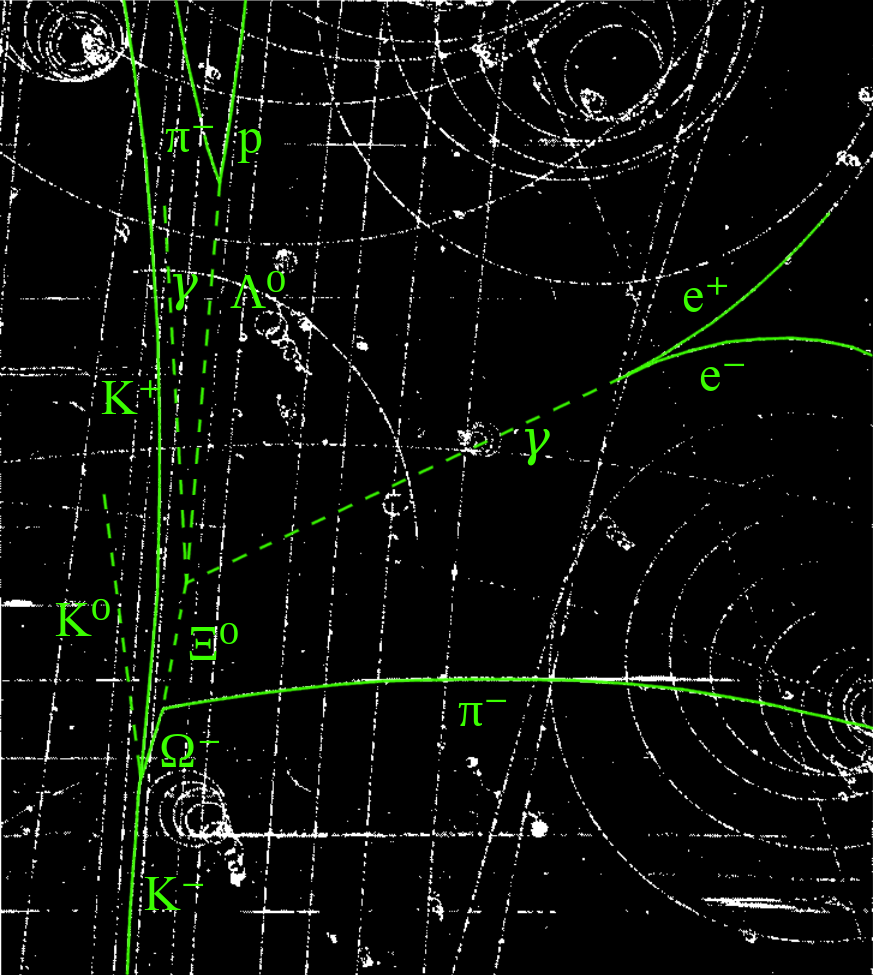
\includegraphics[width=\linewidth]{img/omega-minus-2.png}
\column{0.55\linewidth}

\begin{center}
In 1964, a group at Berkeley sifted through 100,000 photos to find this one: tracks left by decay products of an $\Omega$ baryon.

\vspace{0.25 cm}
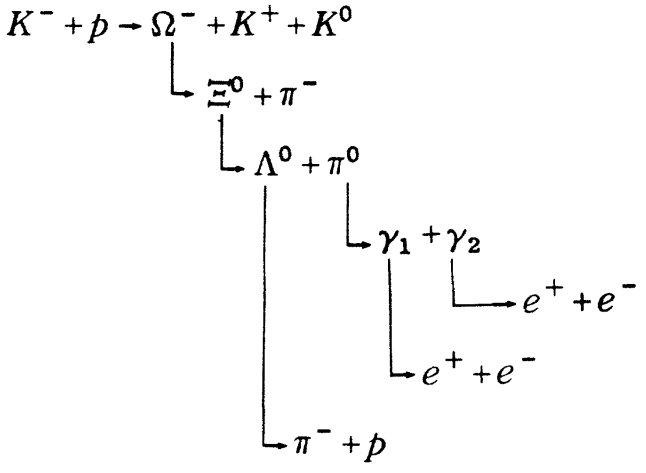
\includegraphics[width=\linewidth]{img/decay-chain.png}
\end{center}

\end{columns}
\end{frame}

\begin{frame}{Today: the same {\it kind} of thing, but bigger}
\vspace{0.15 cm}
\begin{columns}
\column{0.32\linewidth}
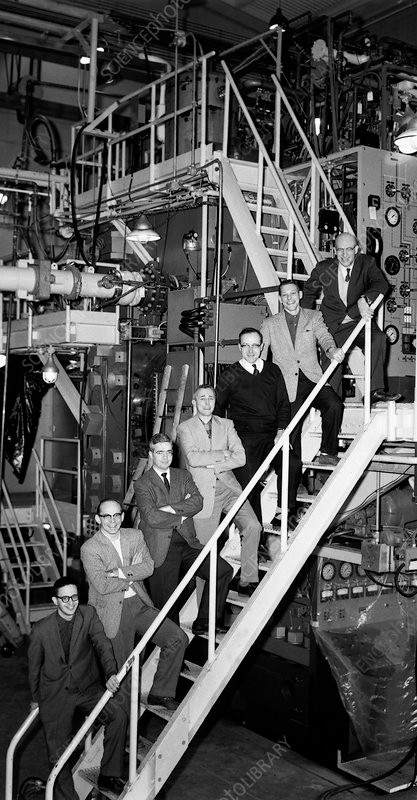
\includegraphics[width=\linewidth]{img/H4000010-Team_that_discovered_Omega_minus_particle.jpg}

\column{0.5\linewidth}
\begin{center}
\begin{columns}
\column{0.35\linewidth}
\centering
\vspace{-1 cm}

photographs

\vspace{\baselineskip}
\vspace{0.5 cm}
100,000 events

\vspace{0.5 cm}
manual/semi-automated scans

\vspace{\baselineskip}
\vspace{0.5 cm}
30 authors

\column{0.35\linewidth}
\centering
\vspace{-1 cm}

digitized signals \\

\vspace{0.5 cm}
$\sim$trillion events \\

\vspace{0.5 cm}
algorithmic searches and machine learning

\vspace{0.5 cm}
3,000 authors
\end{columns}
\end{center}

\column{0.32\linewidth}
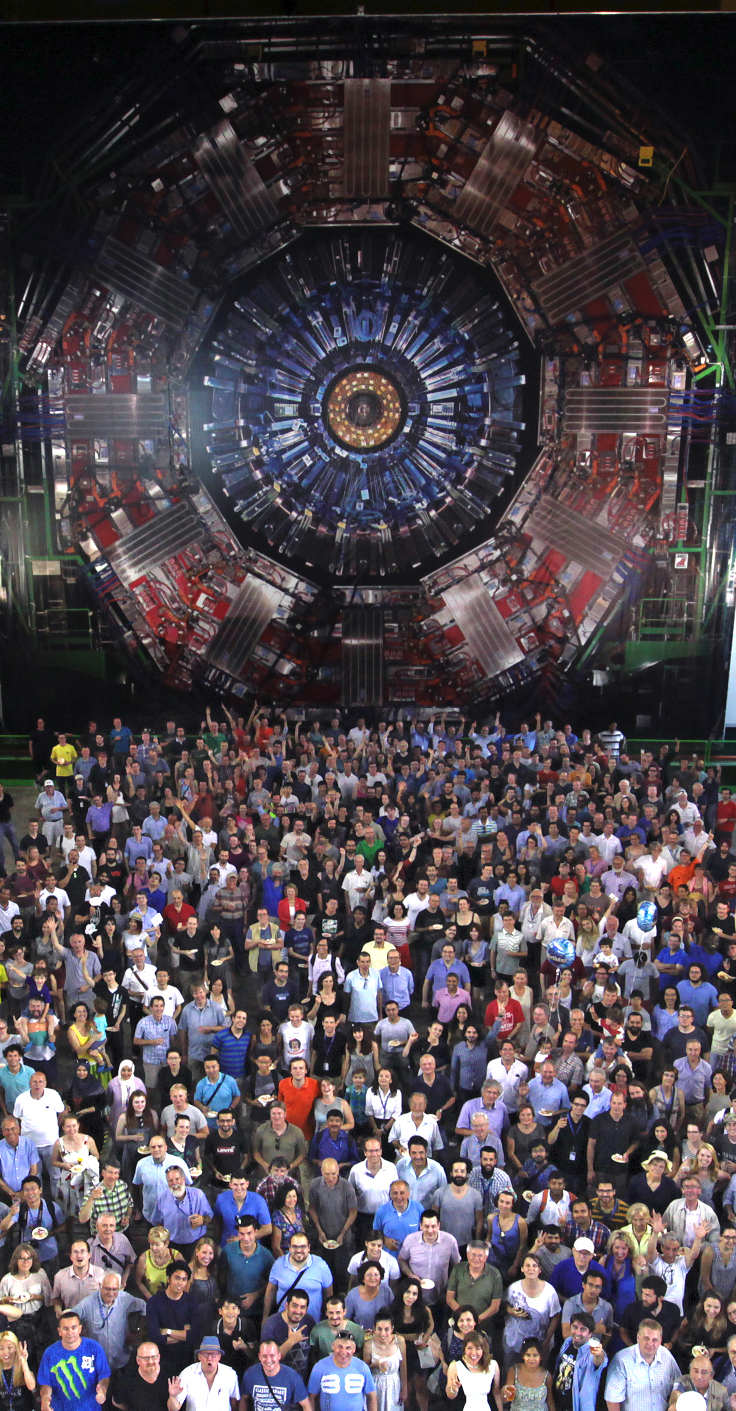
\includegraphics[width=\linewidth]{img/cms25_2.jpg}
\end{columns}
\end{frame}

\begin{frame}{}
\Large
\begin{columns}
\column{1.15\linewidth}
\vspace{-0.5 cm}
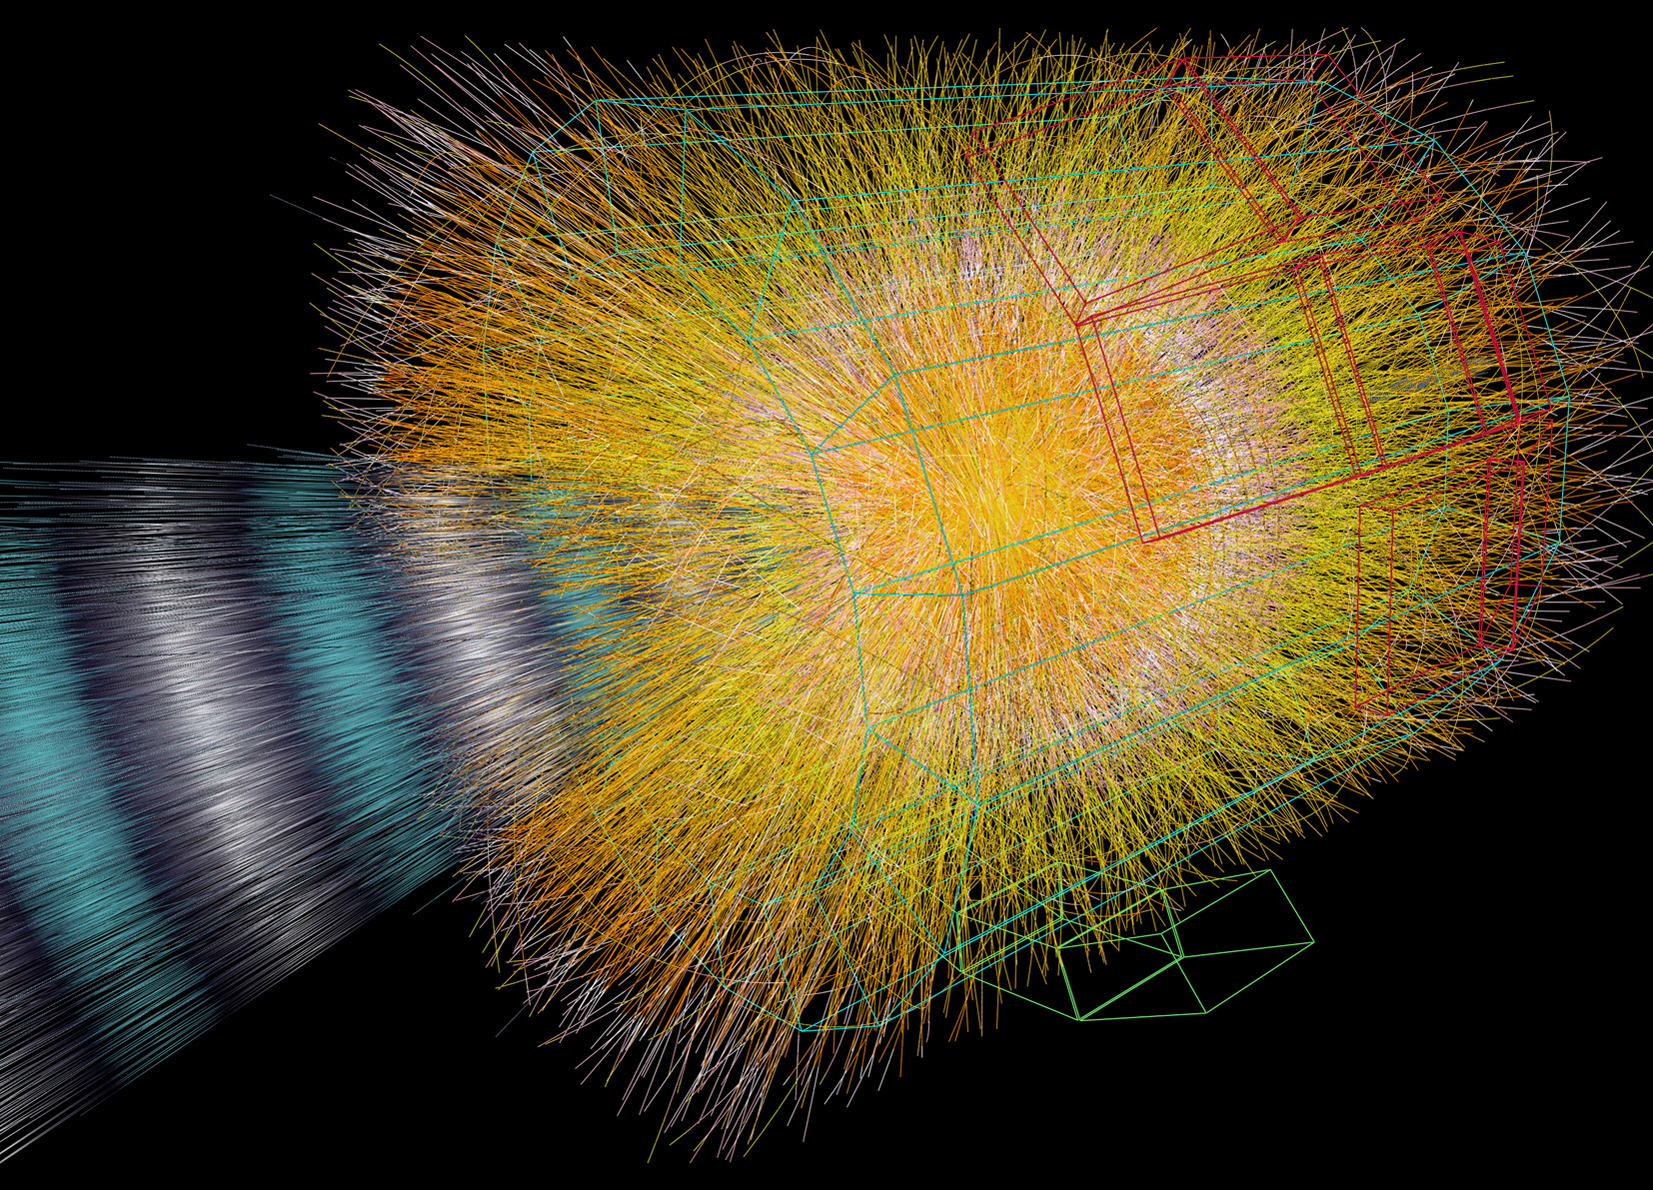
\includegraphics[width=\linewidth]{img/090324_ALICE-hirez.jpg}

\vspace{-11 cm}
\textcolor{white}{\hspace{0.25 cm} Combinatorics problem: tracks aren't labeled!}

\vspace{11 cm}
\end{columns}
\end{frame}

\begin{frame}{Finding a decay: ${K^0}_s \to \pi^+\pi^-$ example}
\large
\vspace{0.5 cm}
\begin{enumerate}
\item Loop over all pairs of particle tracks, tentatively labeling them $\pi^+$ and $\pi^-$.
\item Calculate $m = \sqrt{(E_{\pi^+} + E_{\pi^-})^2 - \left|\vec{p}_{\pi^+} + \vec{p}_{\pi^-}\right|^2}$ for each pair.
\end{enumerate}

\begin{center}
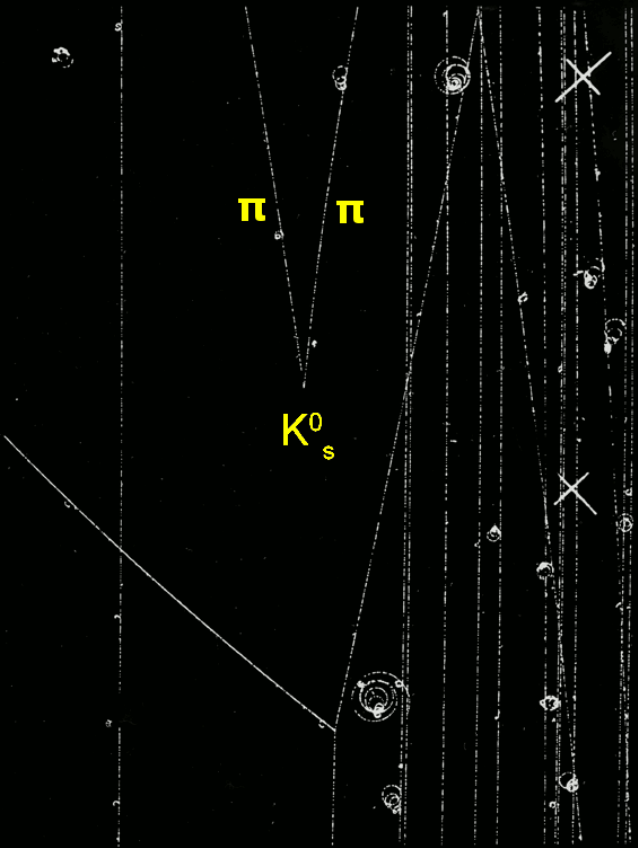
\includegraphics[height=4.2 cm]{img/kshort-1.png}\hspace{0.1 cm}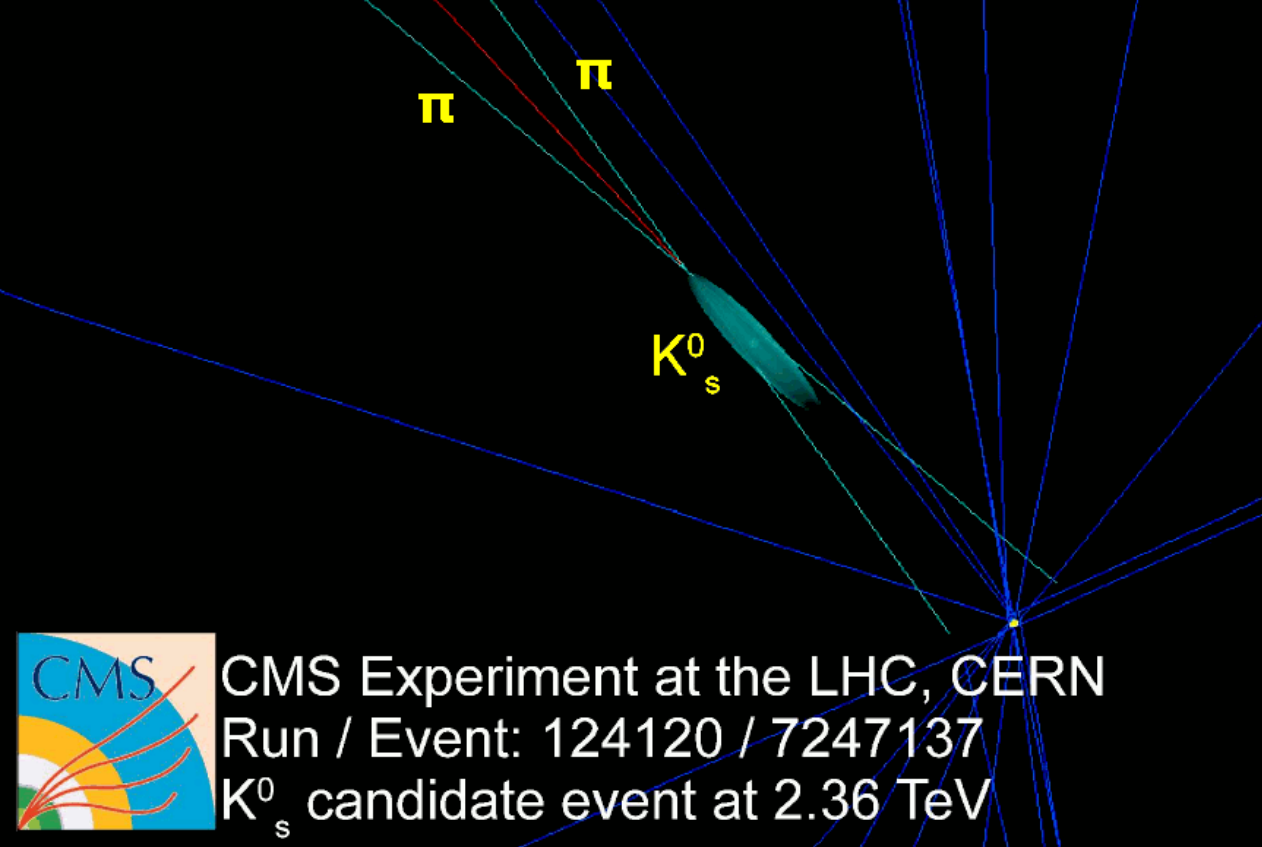
\includegraphics[height=4.2 cm]{img/kshort-2.png}\hspace{0.1 cm}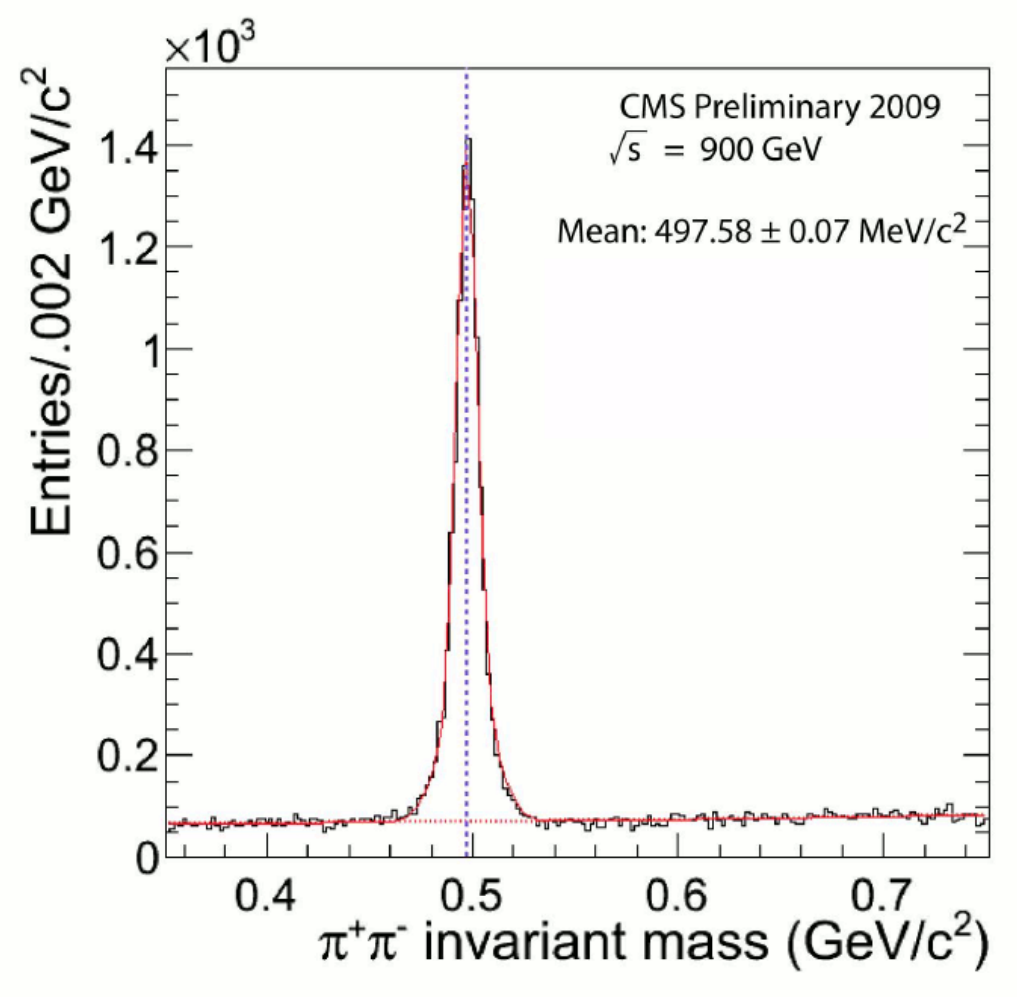
\includegraphics[height=4.2 cm]{img/kshort-3.png}
\end{center}

\begin{enumerate}\setcounter{enumi}{2}
\item The ones with $m \sim \mbox{mass}({{K^0}_s}) = 0.5\mbox{ GeV}/c^2$ are good candidates.
\end{enumerate}
\end{frame}

\begin{frame}{Apply the technique successively down the decay chain}
\Large
\begin{center}
$H \to ZZ$\hspace{1 cm}$Z \to e^+e^-$\hspace{1 cm}$Z \to \mu^+\mu^-$
\end{center}

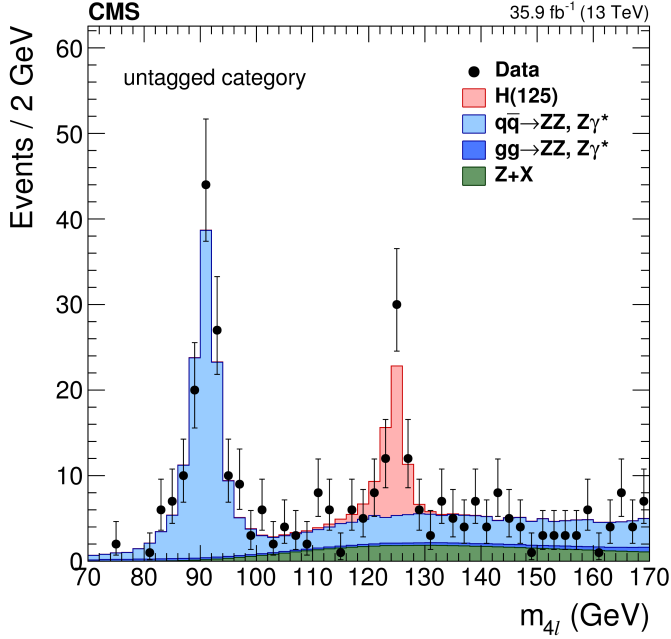
\includegraphics[height=6 cm]{img/higgs-to-four-leptons.png}\hfill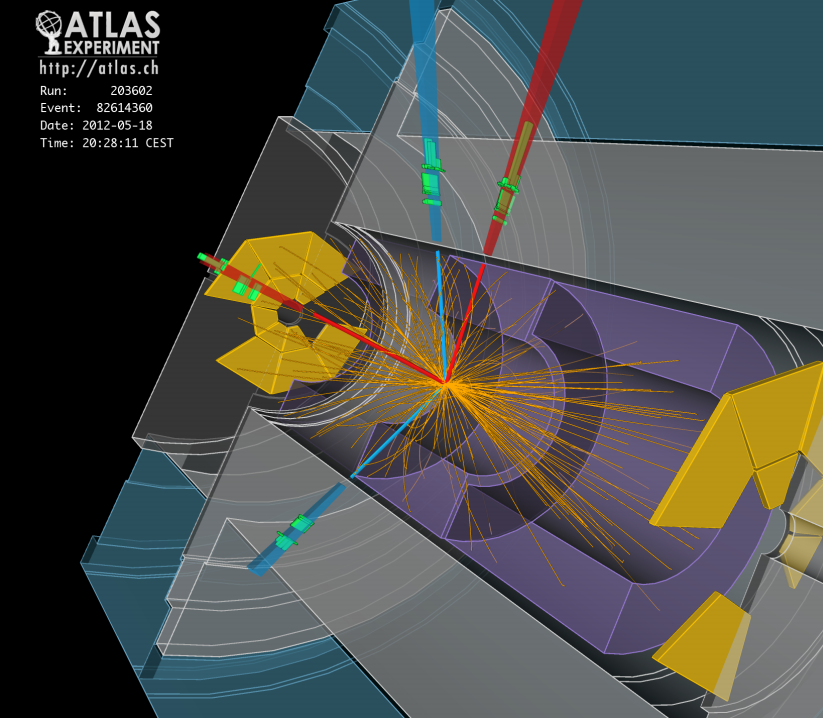
\includegraphics[height=6 cm]{img/higgs-to-four-leptons-2.png}
\end{frame}

\begin{frame}{Data structures are essential for this (and always have been)}
\large
\vspace{0.5 cm}

\vspace{0.25 cm}
\textcolor{darkblue}{{\it Initiation to Hydra} by R.K. B\"ock, 1976: added data structures to Fortran.}

\begin{center}
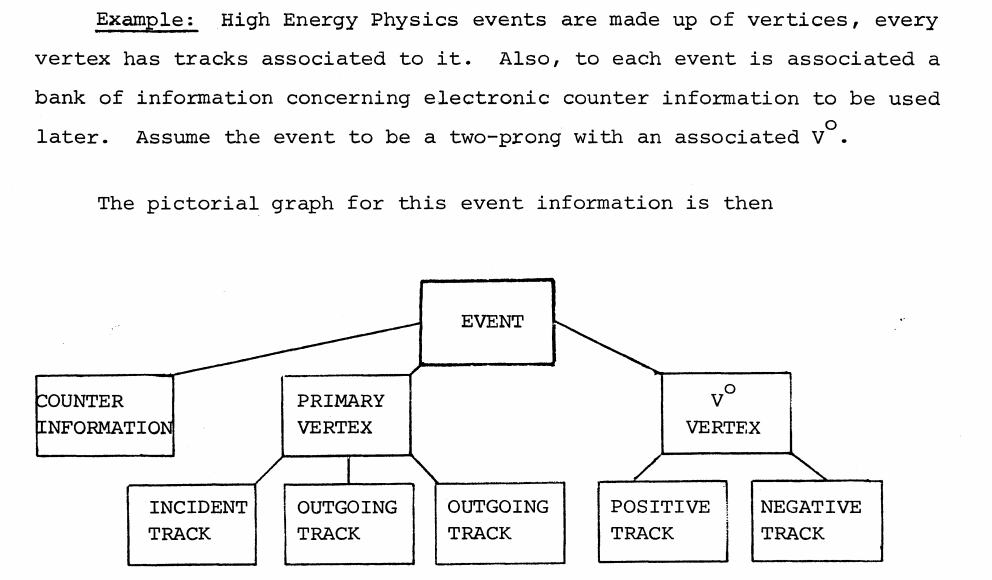
\includegraphics[width=0.7\linewidth]{img/hydra-3.png}
\end{center}
\end{frame}

\begin{frame}{Today, physicists use C++ and Python for analysis}
\large
\vspace{0.25 cm}

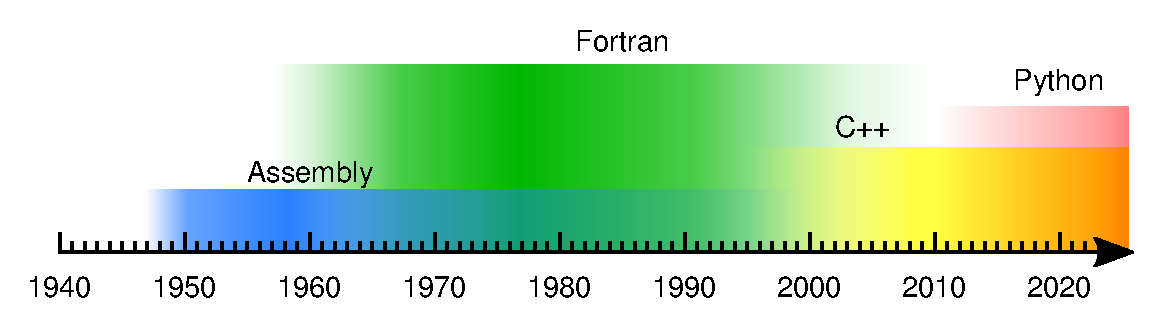
\includegraphics[width=\linewidth]{img/programming-languages.pdf}

\vspace{0.2 cm}
\begin{itemize}\setlength{\itemsep}{0.2 cm}
\item<2-> In C++, we can just write \mintinline{c++}{for} loops over data structures.
\item<3-> In Python, we have a difficult choice: NumPy is fast but limited to rectangular structures; pure Python is slow, but general.
\end{itemize}

\vspace{0.2 cm}
\Large
\begin{center}
\begin{minipage}{0.85\linewidth}
\begin{center}
\uncover<4->{Awkward Array provides NumPy-like interface and performance for general data structures.}
\end{center}
\end{minipage}
\end{center}
\end{frame}

\begin{frame}{}
\Huge
\vspace{1 cm}
\begin{center}
\textcolor{darkblue}{Exploring a dataset: Chicago bike paths}
\end{center}
\end{frame}

\begin{frame}{}
\Huge
\vspace{1 cm}
\begin{center}
\textcolor{darkblue}{Data types and extending NumPy}
\end{center}
\end{frame}

\begin{frame}{Data types \only<6->{and array features}}
\Large
\vspace{0.2 cm}

\begin{itemize}
\item<1-> \textcolor{darkblue}{Numerical:} what \mintinline{python}{np.ndarray} does: numbers, booleans, anything fixed-width.
\item<2-> \textcolor{darkblue}{Variable-length lists:} also known as ``jagged'' or ``ragged'' arrays.
\item<3-> \textcolor{darkblue}{Nested records:} with named (dict) or unnamed (tuple) fields.
\item<4-> \textcolor{darkblue}{Option type:} nullable/masked data; values that can be \mintinline{python}{None}.
\item<5-> \textcolor{darkblue}{Union type:} heterogeneous data; different types in one array.
\end{itemize}

\vspace{0.25 cm}
\begin{itemize}
\item<6-> \textcolor{darkblue}{Indirection:} can be used to enumerate categorical values.
\item<7-> \textcolor{darkblue}{Partitioning:} chunks of an array can be processed in parallel.
\item<8-> \textcolor{darkblue}{Virtualness:} they can also be lazily loaded.
\item<9-> \textcolor{darkblue}{Behaviors:} arrays and records with domain-specific meaning, like ``spacetime point'' or ``string'' can be given specialized methods.
\end{itemize}
\end{frame}



\end{document}
